 


\section{Q1}
\label{part1}
\begin{enumerate}


\item Using the pages from A3 that boilerpipe successfully processed, download those representations again and reprocess them with boilerpipe.
\subitem 1.1 Document the time difference (e.g., Time(A4) - Time(A3)).
\subitem 1.2 Compute the Jaccard Distance x for each pair of pages (i.e., P(A3) and P(A4) for:
\subsubitem - Unique terms (i.e., unigrams)
\subsubitem - Bigrams
\subsubitem - Trigrams

\subitem 1.3 See:  \url{http://en.wikipedia.org/wiki/Jaccard_index}
- WSDM 2010 paper: \url{http://www.l3s.de/~kohlschuetter/boilerplate/}

\subitem 1.4 For each of the 3 cases (i.e., 1-, 2-, 3-grams) build a Cumulative Distribution Function that shows the percentage change on the x-axis and the percentage of the population on the y-axis

\subitem 1.5 See: \url{http://en.wikipedia.org/wiki/Cumulative_distribution_function}

\end{enumerate}

\subsection{Solution}

\begin{enumerate}

\item Time difference between the two sets of boilerpipe representations of the HTML documents is one month.

\item I already had one set of boilerpipe representations of these HTML documents from A3.

\item I used the same python program using `boilerpipe' library from A3 to fetch just the text from the same 10,000 URIs of A3.

\item Next, I wrote a python program to find the unigram, bigrams and trigrams and find the Jaccard Distance x for each pair of pages (i.e., P(A3) and P(A4)). To find unigram, bigrams and trigrams
I used `nltk' library.

\item Following table lists few examples which shows the range of change measured:

\begin{figure}[ht]    
    \begin{center}
        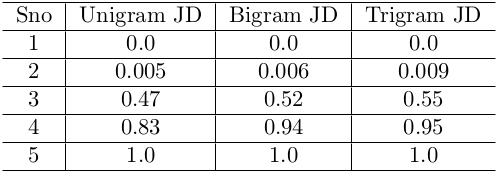
\includegraphics[scale=0.60]{src/examples.png}
        \caption{Examples}        
    \end{center}
\end{figure}

    %\begin{table}
     %       \caption{Examples}
      %          \begin{center}
       %             \begin{tabular}{ c | c | c | c}
		%			\hline
%Sno & Unigram JD & Bigram JD & Trigram JD \\ \hline
%1 & 0.0 & 0.0 & 0.0 \\ \hline
%2 & 0.005 & 0.006 & 0.009 \\ \hline
%3 & 0.47 & 0.52 & 0.55 \\ \hline
%4 & 0.83 & 0.94 & 0.95 \\ \hline
%5 & 1.0 & 1.0 & 1.0 \\ \hline
%				\end{tabular}
%			\end{center}  
%	\end{table}  


\end{enumerate}

\newpage



\subsection{Code Listing}

\subsubsection{extractTextWithBoilerpipe.py}
\lstinputlisting[language=Python,breaklines = true,frame=single,caption={Python program to extract only text from HTML documents using boilerpipe}, label=lst:q1-1,captionpos=b,numbers=left,showspaces=false,showstringspaces=false,basicstyle=\footnotesize]{src/1.extractTextWithBoilerpipe.py}
\newpage

\subsubsection{findNgrams.py}
\lstinputlisting[language=Python,breaklines = true,frame=single,caption={Python program to calculate jacard distance for Unigram, Bigrams and Trigrams}, label=lst:q1-1,captionpos=b,numbers=left,showspaces=false,showstringspaces=false,basicstyle=\footnotesize]{src/1.findNgrams.py}
\newpage















